\documentclass{beamer}

% \usepackage[british]{babel}
\usepackage[utf8]{inputenc} % This package will support Turkish chars
\usepackage{bilkentbeamer} % beamer style
\usepackage{graphicx,hyperref,url}
\usepackage{amsmath} % mathematics.
\usepackage{amssymb} % symbols
\usepackage{stmaryrd} % some CS related symbols
\usepackage{color}

% Some useful colors
\colorlet{darkblue}{blue!70!black}
\colorlet{darkgreen}{green!70!black}
\colorlet{darkred}{red!70!black}

% Put this preamble if you want to show at the beginning of each section 
% where the current section is in the outline.
% \AtBeginSection[]
% {
%   \begin{frame}
%     \frametitle{Outline}
%     \tableofcontents[currentsection]
%   \end{frame}
% }


% The title of the presentation:
%  - first a short version which is visible at the bottom of each slide;
%  - second the full title shown on the title slide;
\title[Bottom of the Slide Title]{Full Title}

% Optional: a subtitle to be displayed on the title slide
\subtitle{subtitle}

% The author(s) of the presentation:
%  - again first a short version to be displayed at the bottom;
%  - next the full list of authors, which may include contact information;
\author[Alican Büyükçakır]{
  Alican Büyükçakır \\\medskip
  {\small \url{alicanbuyukcakir@bilkent.edu.tr}} \\ 
  {\small \url{http://abuyukcakir.github.io}}}

% The institute:
%  - to start the name of the university as displayed on the top of each slide
%    this can be adjusted such that you can also create a Dutch version
%  - next the institute information as displayed on the title slide
\institute[Bilkent University]{
  Bilkent Information Retrieval Group -- Computer Engineering Department \\
  Bilkent University}

% Add a date and possibly the name of the event to the slides
%  - again first a short version to be shown at the bottom of each slide
%  - second the full date and event name for the title slide
\date[22 Oct 2018]{
  Event Name, City, Country. \\
  22 Oct 2018}

\begin{document}

\begin{frame}
  \titlepage
\end{frame}

\begin{frame}
  \frametitle{Outline}

  \tableofcontents
\end{frame}

% Section titles are shown in at the top of the slides with the current section 
% highlighted. Note that the number of sections determines the size of the top 
% bar, and hence the university name and logo. If you do not add any sections 
% they will not be visible.
\section{Introduction}

\subsection{Motivation}
\begin{frame}
  \frametitle{Motivation}
  Lorem ipsum dolor sit amet?
  
\end{frame}

\begin{frame}{Challenges of Data Streams}
    Data streams are environments where vast amounts of (possibly infinite) data are generated at high speed. Challenges \cite{bifet2009new}:
    \begin{enumerate}
        \item Can see the data once and only once.
        \item Should be able to predict at any time.
        \item Memory constraint.
        \item Robustness to concept drifts.
    \end{enumerate}
\end{frame}

\begin{frame}{Multi-label Classification}
  When a data instance is classified into:
  
  \begin{itemize}
    \item just one label $\lambda \in \mathcal{L}$: single-label classification.
    \item one or more (a subset of) labels $L^* \subseteq \mathcal{L}$: multi-label classification (MLC).
    \begin{itemize}
        \item For $L$-many labels, $2^L$ possible label sets. Combinatorial explosion?
    \end{itemize}
  \end{itemize}
  
  \begin{examples}
  Gene function prediction, text categorization and tagging, movie genre classification, image scene classification, ...
  \end{examples}
\end{frame}

\subsection{Problem Definition}
\begin{frame}{Problem Definition}
    You can insert figures as follows...
    
    \begin{figure}
        \centering
        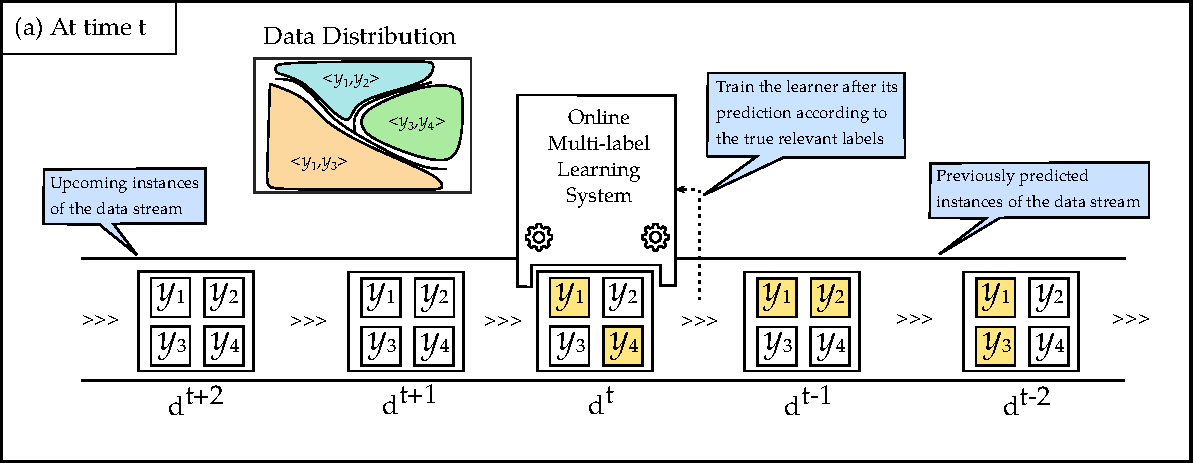
\includegraphics[width=\columnwidth]{images/multi-label-stream-classification-fig1.pdf}
        \caption{MLSC task. with $L=4$. Labels predicted as relevant are filled with yellow. Also, see ITTT (interleaved-test-then-train).}
        \label{fig:mlsc}
    \end{figure}
\end{frame}

\section{Related Work}

\begin{frame}{Related Work}
    We need to know two things:
    
    \begin{enumerate}
        \item How are multi-label problems tackled in general?
        \item What do the ensembles in MLSC task generally do?
    \end{enumerate}
\end{frame}


\section{Main Work}

\subsection{The Idea}

\begin{frame}
  \frametitle{Main Work}

   \begin{alertblock}{Alert Block Title}
Alert block has a title and it s red.
\end{alertblock}

\begin{block}{The basis}
Block is of the same color of the presentation itself.
Can also use items in blocks
\begin{itemize}
  \item split
  \item whale
  \item rounded
  \item orchid
\end{itemize}
\end{block}


\end{frame}

\subsection{Another Subsection}


\section{Experiments and Results}

\begin{frame}{Statistical Significance}
    We used Friedman test with Nemenyi post-hoc analysis \cite{demvsar2006statistical}.
\end{frame}

\section{Discussion and Conclusion}

\begin{frame}
  \frametitle{Discussion}

  \begin{itemize}
    \item Easy to use
    \item Good results
  \end{itemize}
\end{frame}

% \section{References}

% Put references into a 'tiny' group so that more than 3 references can fit into one page.
\begingroup
\tiny   % or you can use: Tiny, small, Small
\begin{frame}[allowframebreaks] %with allowframebreaks, references are divided into pages automatically.
    \frametitle{References}
    \bibliographystyle{apalike}
    \bibliography{bibliography} 
\end{frame}
\endgroup

\end{document}
